% !TEX root = ../IS.tex
\chapter{Extensive Form Games}
\section{Basics of Game Theory}
\section{Normal Form Games}
In the vast majority of human choices, a person will attempt to maximize their utility function; they will perform actions that benefit themselves. When there are two or more agents trying to maximize their utility, the interactions and choices between these agents, or players, become more and more complex. These interactions can be studied with game theory using the normal or strategic form.
\begin{define}
  A finite normal-form game is a tuple $(N, A, u)$ where:
  \begin{itemize}
  \item $N$ is a finite set of $n$ players, indexed by $i$
  \item $A=A_1\times\cdots\times A_n$, where $A_i$ is a finite set of actions available to player $i$. Each vector $a=(a_1,\cdots ,a_n)\in A$ is called an action profile.
    \item $u=(u_1,\cdots ,u_n)$ where $u_i : A \mapsto\mathbb{R}$ is a real-valued utility function for player $i$.
\end{itemize}
\end{define}

In an arbitrary normal-form game, there are $n$ different players contained in the set $N$, where $n$ is a positive integer. For each of these players, there is also a finite set of actions that they can take. Player $N_i$ will have the action set $A_i$. The complete action set $A$ is determined by the Cartesian product of the action sets of each player. Within $A$, a vector $a$ is the action profile; an action profile, or outcome, represents the choice that each player made \cite{osbo94}. The collection of mappings $u$ gives each action profile a particular value; these values determine which outcome is preferred by a player. In normal-form games, players are utility-maximizing agents; they will gravitate towards action profiles which give them higher utility.\\

The normal-form game can be seen in the quintessential ``Prisoner's Dilemma'' example. This game is expressed in a 2x2 matrix, with one player's choices represented in the columns and the other player's choices represented in the rows of said matrix.

\begin{figure}[h]
  \centering
  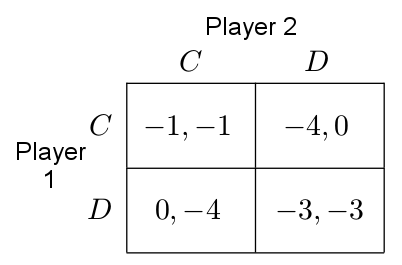
\includegraphics[width=5cm]{OtherFiles/ExampleGrid.png}
  \caption{The Prisoner's Dilemma, represented in a normal form matrix \cite{shoh09}.}
  \label{fig:prisoner}
\end{figure}

In Figure \ref{fig:prisoner}, the column labeled \textit{C} represents prisoner 2 confessing to the crime, while the column labeled \textit{D} represents prisoner 2 denying their guilt. The rows \textit{C} and \textit{D} represent the same choices for prisoner 1. For this game, $A_i$ would be the set $\{C, D\}$, as those are the two choices that each prisoner can make. The element pairs of the matrix are the utility function of each player. In this case, their utility is the number of years in jail to which a player will be sentenced. The mapping functions in $u$ correspond to the leniency of the courts. When both deny committing the crime, the prisoners each get three years in prison. If both confess to the crime, they both get one year in prison; their sentence is lighter for cooperating with the police. If only one prisoner confesses, that player gets a four year sentence, while the player who denied gets no time in jail.\\

\_\_\_\_\_\_ Nash Equillibria

\_\_\_\_\_\_ Put a proof in here, possibly

It is important to recognize in this example that the two prisoners are making their choice simultaneously. For games with sequential actions, the normal form is no longer sufficient to represent player choices. Instead, games with sequential actions are represented in extensive-form trees.\\

\_\_\_\_\_\_ Make a more complicated example to segue into 2.1, and reword previous paragraph
\section{Extensive Form Trees}
\_\_\_\_\_\_ Intoduction paragraph
\begin{define}
  A finite perfect information game in extensive form is a tuple $G = (N, A, H, Z, \chi, \rho, \sigma, u)$ where:
  \begin{itemize}
  \item $N$ is a set of n players;
  \item $A$ is a single set of actions;
  \item $H$ is a set of non-terminal, choice nodes;
  \item $Z$ is a set of terminal nodes, disjoint from $H$;
  \item $\chi: H\mapsto 2^A$ is the action function, mapping a set of possible actions to each choice node;
  \item $\rho: H\mapsto N$ is the player function, mapping to each non-terminal node a player who makes an action at said node;
  \item $\sigma: H\times A\mapsto H\bigcup Z$ is the successor function, mapping a choice node and an action to a new choice or terminal node. $\forall h_1, h_2\in H$ and $a_1, a_2\in A$, if $\sigma(h_1, a_1)=\sigma(h_2, a_2)$, then $h_1=h_2$ and $a_1=a_2$;
  \item $u=(u_1,...,u_n)$, where $u_i:Z\mapsto \mathbb{R}$ is a real-valued utility function for each player $i$ on a terminal node $Z$
  \end{itemize}
\end{define}

\begin{figure}[h]
  \centering
  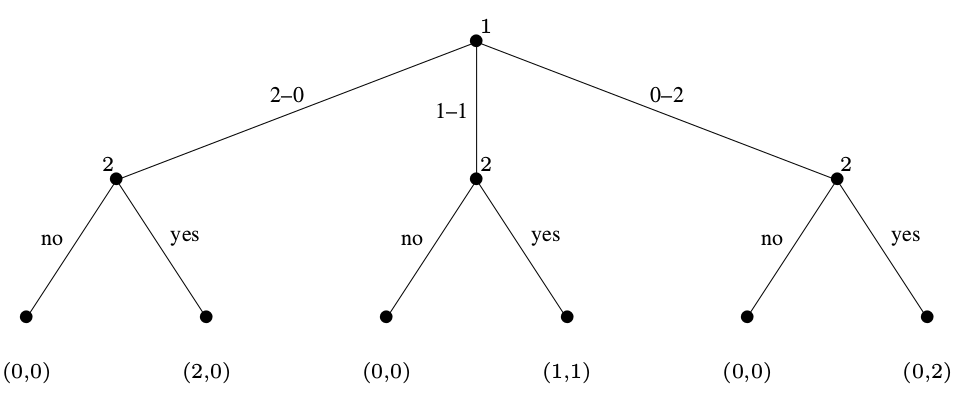
\includegraphics[width=10cm]{OtherFiles/ExampleTree.png}
  \caption{An extensive-form tree for The Sharing Game}
  \label{fig:sharingTree}
\end{figure}

To explore this definition, take the game of tic-tac-toe. Let $N={N_1, N_2}$ be the set of players in the game. For the first move of the game, $A$ is the set of 9 open spaces on the board; for the second move, $A$ is the set of the remaining 8 spaces. For a game of tic-tac-toe, $H$ contains configuration of the board where neither player has three in a row and there are still open squares on the board. $Z$, on the other hand, contains the board configurations where one player has three in a row or all spaces have been claimed. For tic-tac-toe, the $\chi$ function removes illegal actions from a node, which in tic-tac-toe would be playing on an occupied square. Thus, the $\chi$ function leaves the choice nodes at each successive turn with fewer and fewer available actions. Since there are only two players, the $\rho$ function alternates between players after each action.